\section{Teórico}

  \definicion{Topic:} Introduction to Magnetism.

  \definicion{Speaker:}	Alessandro STROPPA (CNR-SPIN, Italy).

\subsection{Integrales de Coulomb y de intercambio}

  La integral de Coulomb $I$ es una cantidad positiva que hace referencia a la repulsión electrostática entre las densidades electrónicas $\norm{\psi_{100} (\vec{r}_1)}^2$ y $\norm{\psi_{nlm} (\vec{r}_2)}^2$; en cambio, la integral de intercambio $J$ es la energía asociada al intercambio de los estados cuánticos entre 2 electrones. El valor de $J$ puede ser negativo (antiparalelos) o positivo (paralelos).

  En el caso del singlete la repulsión Coulómbica tiende a ser mayor debido a que los electrones están más cercanos entre sí. La diferencia etre el estado single y el triple es $2J$.
    \begin{figure}[H]
        \centering
        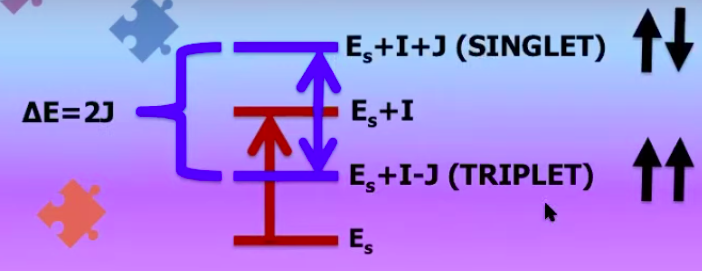
\includegraphics[scale = 0.6]{figs/D7/IJ.png}
    \end{figure}

  Cuando consideramos la interacción Coulómbica interelectrónica junto al postulado de simetrización llegamos al intercambio. Luego, partiendo desde un Hamiltoniano que no depende del spin podemos llegar a interacciones spin-dependientes.

\subsection{Interacción spin-órbita}

  La interacción spin-órbita (SO) es el acople entre el momento angular de spin $\vec{s}$ y el momento angular orbital $\vec{l}$. Esta interacción es unas 10 a 100 veces menor que el intercambio. A pesar de ser tan pequeña su  contribución es muy importante para el magnetismo.

  La energía magnética es $E = - \vec{m}_S \cdot \vec{B}_L$ y, como $\vec{m}_S \propto \vec{s}$ y $\vec{B}_L \propto \vec{l}$, entonces $E \propto \vec{s} \cdot \vec{l}$. El splitting generado por el acople SO puede ir desde los $10^{-5}$ eV para átomos livianos hasta los 0.1-1 eV para átomos pesados.

  La importancia del acople SO es que determina la anisotropia magnetocristalina en sólidos.

\subsection{High vs low spin}

  Al combinar el principio de exclusión de Pauli con las reglas de Hund, obtenemos dos situaciones:
    \begin{itemize}
      \item \textbf{High spin:} cuando la interacción $J$ es mayor que el splitting generado por el campo ligando, es preferible llenar la mayor cantidad de orbitales con igual spin (incluyendo orbitales de alta energía) antes de comenzar a utilizar el spin opuesto.
      \item \textbf{Low spin:} cuando la interacción $J$ es menor que el splitting generado por el campo ligando, es preferible llenar sólo los orbitales de menor energía.
    \end{itemize}

    \begin{figure}[H]
        \centering
        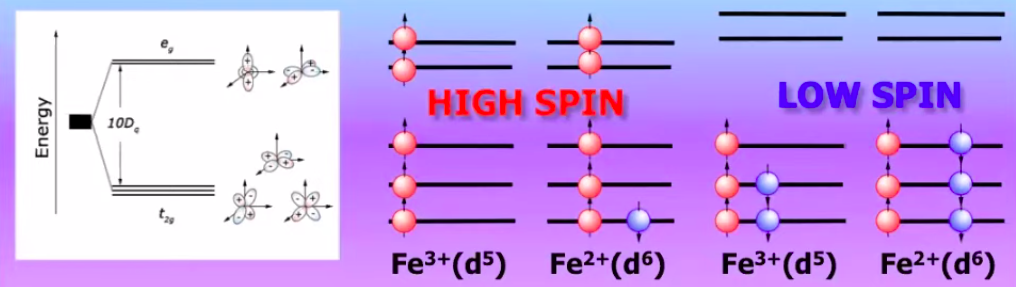
\includegraphics[scale = 0.5]{figs/D7/highlow.png}
    \end{figure}

\subsection{Potencial centrífugo: magnetismo localizado vs itinerante}

  Los electrones internos determinan el potencial sobre el cual se mueven los electrones externos. Este potencial central depende del momento angular orbital: a mayor $l$, más atrapados (localizados) estarán los electrones. Esto da lugar a la localización en los electrones 3d de los metales de transición y en los 4fde las tierras raras.

\subsection{Modelo de Stoner}

  Se trata del modelo de bandas más sencillo utilizado para explicar el ferromagnetismo en metales. La interacción entre los electrones 3d provoca un smearing de su energía, dando lugar a una banda, la cual puede describirse con DFT. Al considerar la energía media de los estados de la banda de valencia se puede aproximar la DOS mediante un semicírculo.

    \begin{figure}[H]
        \centering
        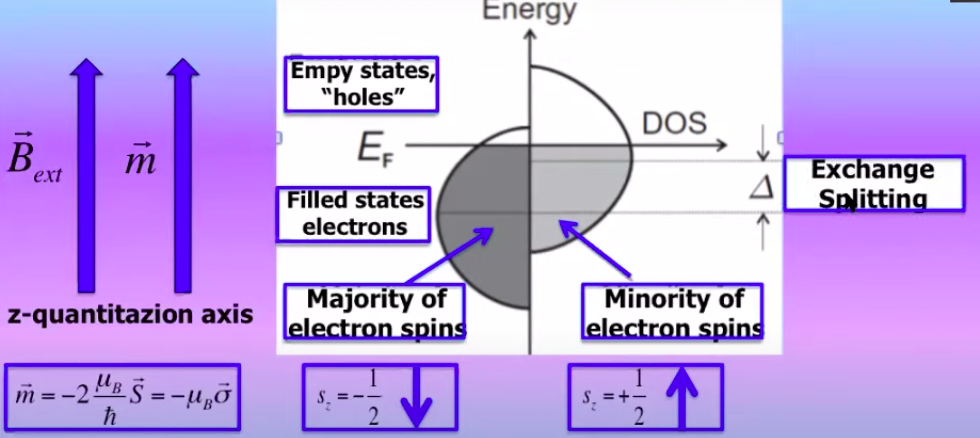
\includegraphics[scale = 0.5]{figs/D7/stoner.png}
    \end{figure}

\subsection{Magnetismo colinear y no colinear}

  En el caso no colineal no existe un único eje de cuantización principal, por lo que se deben generar CL entre los spins up y down; en cambio, en el caso colineal sí se tiene un único eje de cuantización principal permitiendo tener por un lado la contribución up y por otra parte la contribución down.

  \begin{figure}[H]
      \centering
      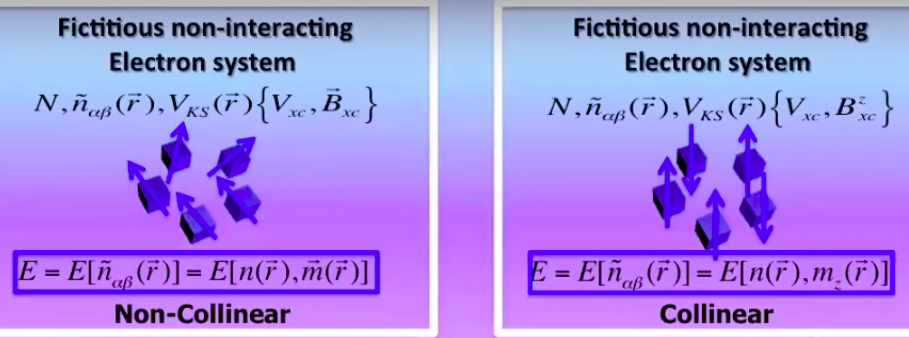
\includegraphics[scale = 0.5]{figs/D7/colin.png}
  \end{figure}

  Al final de cuentas tenemos que:
    \begin{itemize}
      \item La densidad de carga es la suma de las contribuciones up y down de la función de onda.
      \item La densidad de spin en $z$ es la resta de las contribuciones up y down de la función de onda.
      \item La densidad de spin en $x$ y en $y$ son la parte real y la parte imaginaria, respectivamente, del producto entre la función de onda y su conjugada, ambas con spins opuestos.
    \end{itemize}

\subsection{Spin DFT}

  Para hacer DFT considerando el spin hay que extender las ecuaciones KS a sistemas spin-polarizados, introduciendo una matriz 2x2 para la densidad electrónica. A partir de esto, las densidades y los potenciales se pueden descomponer como CL de las matrices de Pauli: la contribución escalar viene de DFT sin spin mientras que la contribución vectorial viene de la mano del magnetismo.

  En QE podemos obtener:
    \begin{itemize}
      \item Energía total (pw-scf).
      \item Momento magnético de spin total y absoluto  (pw-scf).
      \item Estructura de bandas (pw-nscf), tanto para el caso de spins no polarizados como para polarización colineal y no colineal.
      \item DOS (pw-nscf): DOS total o local.
      \item Momentos locales.
    \end{itemize}

\section{Q\&A}

  \definicion{can we calculate the exchange interaction using QE?}

  You may extract exchange interactions by fitting your results to some suitable spin hamiltonian; or, if you know the integrals to be computed, you can use data from QE to compute them. QE doesn't directly do that, though.

  \definicion{Why in the magnetic case in 'scf' calculation the flag 'starting\_magnetization' is 0.26, while in the 'nscf' one the flag 'starting\_magnetization' is set to 0.7?}

  It is just an initial guess (the important thing is that it is different from 0.0) and I add, in the ncsf run it does not compute again the magnetic moment- It just reads the charge  density and diagonalize the matrix to compute the dos

  \definicion{If we have 2 atoms in unit cell, we don’t have to specific starting\_magnetization(2)?}

  starting\_magnetization is set PER TYPE OF ATOM, not per atom

\section{Hands-on}

  \definicion{Topic:} Introduction to Magnetism.

  \definicion{Speaker:}	Pietro DELUGAS (SISSA, Italy).

  Se estudia el magnetismo en metales de transición: Fe, Co y Ni.

\subsection{Ex 1}

  Activamos la solución mangética:
  $nspin = 2$ 1 es para no polarizado y 2 es spin polarizado
  $starting\_magnetization$ rompe la simetría entre el up y el down.
  $noncolin=.true.$ sistema no colineal
  $angle$ 1 es el polar y 2 es el acimutal. Necesario para el caso no colineal.
